% (c) 2012-2013 Claudio Carboncini - claudio.carboncini@gmail.com
% (c) 2012-2014 Dimitrios Vrettos - d.vrettos@gmail.com
% (c) 2014 Daniele Zambelli - daniele.zambelli@gmail.com

% (c) 2014 Daniele Zambelli - daniele.zambelli@gmail.com
% 
% Tutti i grafici per il capitolo relativo alle parabole
%
% 

\newcommand{\espdueterzi}{% 
    % Esponenziali con basi diverse.
    \disegno{
    \rcom{-10}{+10}{-1}{10}{gray!50, very thin, step=1}
    \begin{scope}[ultra thick, color=Maroon!50!black]
     \tkzInit[xmin=-10.3, xmax=+10.3, ymin=-0.3, ymax=+10.3]
     \tkzFct[domain=-10.3:+6]{(3./2)**x}
     \tkzFct[color=Green!50!black, domain=-6:+10.3]{(2./3)**x}
     \begin{scope}[color=Black!50!black]
      \filldraw (1, 3./2) circle (1.2pt);
      \filldraw (1, 2./3) circle (1.2pt);
     \end{scope}
     \filldraw [color=Red](0, 1) circle (1.2pt);  
    \end{scope}
    \begin{scope}[color=black]
     \draw (-7.3, 7) node{\(f(x)=\tonda{\dfrac{2}{3}}^x\)}; 
     \draw ((7.3, 7) node{\(f(x)=\tonda{\dfrac{3}{2}}^x\)};
    \end{scope}
    }
}

\newcommand{\logduebasi}{% 
    % Esponenziali con basi diverse.
    \disegno{
    \rcom{-1}{+10}{-9}{9}{gray!50, very thin, step=1}
    \begin{scope}[ultra thick, color=Maroon!50!black]
      \tkzInit[xmin=-1.3, xmax=+80, xstep=.5, ymin=-10.3,ymax=+10.3]
      \tkzFct[domain=.01:+10]{log(x)/log(2)}
      \filldraw (2, 1) circle (1.2pt);
      \begin{scope}[color=Green!50!black]
        \tkzFct[domain=-.01:+10]{log(x)/log(1./2)}
        \filldraw (2, -1) circle (1.2pt);
      \end{scope}
    \end{scope}
    \begin{scope}[color=black]
      \draw (9.5, 2.8) node{a=2}; 
      \draw (9.5, -2.8) node{a=0.5};
    \end{scope}
      \filldraw [color=Red] (1,0) circle (1.2pt);
    }
}


\chapter{Il piano cartesiano}

\section{Un po' di storia}
\label{sec:01_storia}

Nel~$II$~secolo~\aC\ Ipparco compilò il primo catalogo stellare in cui 
precisò la posizione di circa~850 stelle sulla sfera celeste mediante due 
numeri: latitudine e longitudine. La posizione di un punto era dunque 
individuata attraverso una coppia di numeri.
Ancora oggi attraverso latitudine e longitudine viene individuato un punto 
sulla superficie terrestre.
I romani nel fondare una città segnavano due solchi perpendicolari ai quali 
riferivano la posizione di case, monumenti, strade.

Nonostante queste intuizioni, per migliaia di anni la geometria e l'algebra 
sono state due discipline completamente separate nella matematica.

Nel~$XVII$~secolo con le opere di Pierre de Fermat e di René Descartes il 
metodo di rappresentare punti con coppie di numeri. 
Il \emph{piano cartesiano} è uno strumento che permette di trattare elementi 
geometrici con metodi algebrici ed elementi algebrici con metodi geometrici.
Così, a volte,  problemi algebrici difficili possono a trovare una soluzione 
geometrica semplice e viceversa.
In matematica, ma anche nelle altre scienze, quando si riesce a trovare un 
collegamento tra due rami della disciplina che fino a quel momento erano
rimasti separati, si fa un grande passo avanti.

La geometria analitica permette di descrivere enti geometrici attraverso 
numeri, equazioni, disequazioni e tradurre le relazioni tra elementi della 
geometria in relazioni tra enti dell'algebra e viceversa.

\section{Asse cartesiano}
\label{sec:02_asse}

Lo strumento che ci permette di fare tutto ciò è il 
\emph{riferimento cartesiano}. L'idea di base è che su una retta ci sono 
infiniti punti e anche i numeri sono infiniti possiamo quindi far 
corrispondere ai punti della retta tutti gli elementi di un insieme numerico.
Possiamo farlo a fantasia o seguendo un metodo che permette a tutti di 
disporre i numeri esattamente nello stesso modo.

\begin{inaccessibleblock}[Figura: TODO]
 \begin{figure}[h]
 \centering
 \begin{minipage}[t]{.45\textwidth}
  \centering \assea
%   \centering% (c) 2014 Daniele Zambelli - daniele.zambelli@gmail.com

%%%
% Retta con i numeri disordinatiordinati
%%%%
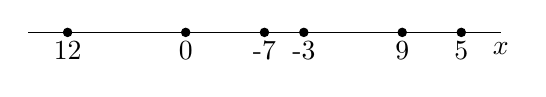
\begin{tikzpicture}[x=5mm, y=5mm, smooth]

\draw [-] (-6,0) -- (6,0) node [below]  {$x$};
\filldraw (-5,0) circle (1.5pt) node [below] {12};
\filldraw (-2,0) circle (1.5pt) node [below] {0};
\filldraw (0,0) circle (1.5pt) node [below] {-7};
\filldraw (1,0) circle (1.5pt) node [below] {-3};
\filldraw (3.5,0) circle (1.5pt) node [below] {9};
\filldraw (5,0) circle (1.5pt) node [below] {5};

\end{tikzpicture}
 \end{minipage}\hfil
 \begin{minipage}[t]{.45\textwidth}
  \centering \asseb
%   \centering% (c) 2014 Daniele Zambelli - daniele.zambelli@gmail.com

%%%
% Retta con i numeri ordinati
%%%%
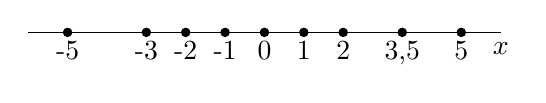
\begin{tikzpicture}[x=5mm, y=5mm, smooth]

\draw [-] (-6,0) -- (6,0) node [below]  {$x$};
\filldraw (-5,0) circle (1.5pt) node [below] {-5};
\filldraw (-3,0) circle (1.5pt) node [below] {-3};
\filldraw (-2,0) circle (1.5pt) node [below] {-2};
\filldraw (-1,0) circle (1.5pt) node [below] {-1};
\filldraw (0,0) circle (1.5pt) node [below] {0};
\filldraw (1,0) circle (1.5pt) node [below] {1};
\filldraw (2,0) circle (1.5pt) node [below] {2};
\filldraw (3.5,0) circle (1.5pt) node [below] {3,5};
\filldraw (5,0) circle (1.5pt) node [below] {5};

\end{tikzpicture}
 \end{minipage}
\end{figure}
\end{inaccessibleblock}

Per farlo in modo preciso abbiamo bisogno di aggiungere ad una retta alcuni 
elementi ottenendo così un asse cartesiano:

\begin{definizione}
  Un \emph{asse cartesiano} è una retta dotata di:
  \begin{itemize} [noitemsep]
   \item \emph{origine}, un punto della retta che rappresenta lo zero, 
    a questo punto normalmente viene dato il nome ``O'';
   \item \emph{verso}, una freccia che indica da quale parte i numeri 
    aumentano;
   \item \emph{unità di misura}, un segmento che indica la distanza tra 
    un numero intero e il successivo.
  \end{itemize}
\end{definizione}

% \begin{center} % (c) 2014 Daniele Zambelli - daniele.zambelli@gmail.com
%%%
% Asse cartesiano vuoto con l'indicazione dell'unità separata
%%%%
\usepgflibrary{arrows.meta}

\begin{tikzpicture}[x=10mm, y=10mm, smooth]

\draw [-{Stealth[length=2mm, open, round]}] (-6.3,0) -- (6.3,0) node [below]  {$x$};
\draw[|-|] (0,.5) -- (1,.5) node[below, midway] {unità};
\filldraw (0,0) circle (1.5pt) node [below] {0};

\end{tikzpicture} \end{center}

\begin{center} \assec \end{center}

Normalmente, invece di indicare l'unità di misura al di fuori dell'asse
indichiamo sull'asse i punti~0~e~1. 

% \begin{center} % (c) 2014 Daniele Zambelli - daniele.zambelli@gmail.com

%%%
% Asse cartesiano con i trattini
%%%%
%\usepgflibrary{arrows.meta}
 
\begin{tikzpicture}[x=10mm, y=10mm, smooth]

%Asse cartesiano con trattini
% (c) 2014 Daniele Zambelli - daniele.zambelli@gmail.com

%%%
% Asse cartesiano con i trattini
%%%%
%Asse cartesiano con trattini
% \usepgflibrary{arrows.meta}

\draw [-{Stealth[length=2mm, open, round]}] (-6.3,0) -- (6.3,0) node [below]  {$x$};
\foreach \xi in {-6, -5, ..., 6}
\draw [-] (\xi, -.05) -- (\xi, .1);
\node [below] at (0, 0) {0};
\node [below] at (1, 0) {1};


\end{tikzpicture} \end{center}

\begin{center} \assed \end{center}

Quando lavoriamo su un foglio a quadretti, indichiamo esplicitamente 
l'unità solo se è diversa dal quadretto e evitiamo anche di tracciare tutti 
i trattini verticali.

% \begin{center} % (c) 2014 Daniele Zambelli - daniele.zambelli@gmail.com

%%%
% Asse cartesiano nei quadretti
%%%%
\usepgflibrary{arrows.meta}

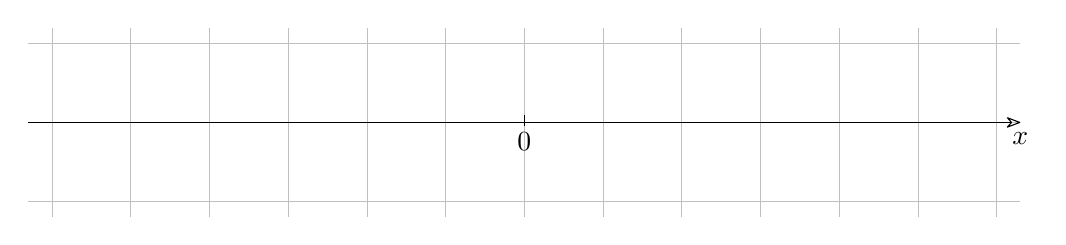
\begin{tikzpicture}[x=10mm, y=10mm, smooth]

%Asse cartesiano nei quadretti
\draw[gray!50, very thin] (-6.3, -1.2) grid (6.3, 1.2);
\draw [-{Stealth[length=2mm, open, round]}] (-6.3,0) -- (6.3,0) node [below]  {$x$};
\draw [-] (0, -.05) -- (0, .1);
\node [below] at (0,0) {0};


\end{tikzpicture} \end{center}

\begin{center} \assee \end{center}

In questo modo possiamo far corrispondere ad ogni numero un punto della retta 
e ad ogni punto della retta un numero \emph{reale}. Il numero che corrisponde 
al punto si chiama \emph{coordinata} del punto.

% \begin{center} % (c) 2014 Daniele Zambelli - daniele.zambelli@gmail.com

%%%
% Asse cartesiano con alcuni esempi di numeri
%%%%

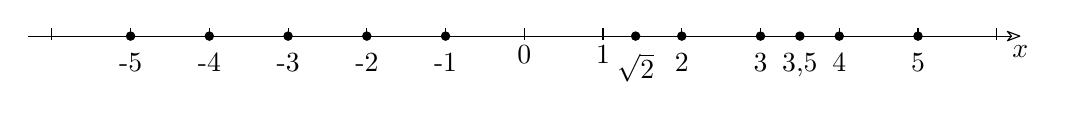
\begin{tikzpicture}[x=10mm, y=10mm, smooth]

%Asse cartesiano con trattini
% (c) 2014 Daniele Zambelli - daniele.zambelli@gmail.com

%%%
% Asse cartesiano con i trattini
%%%%
%Asse cartesiano con trattini
% \usepgflibrary{arrows.meta}

\draw [-{Stealth[length=2mm, open, round]}] (-6.3,0) -- (6.3,0) node [below]  {$x$};
\foreach \xi in {-6, -5, ..., 6}
\draw [-] (\xi, -.05) -- (\xi, .1);
\node [below] at (0, 0) {0};
\node [below] at (1, 0) {1};


\filldraw (-5, 0) circle (1.5pt) node [below, yshift=-.1cm] {-5};
\filldraw (-4, 0) circle (1.5pt) node [below, yshift=-.1cm] {-4};
\filldraw (-3, 0) circle (1.5pt) node [below, yshift=-.1cm] {-3};
\filldraw (-2, 0) circle (1.5pt) node [below, yshift=-.1cm] {-2};
\filldraw (-1, 0) circle (1.5pt) node [below, yshift=-.1cm] {-1};
\filldraw (1.4142, 0) circle (1.5pt) node [below, yshift=-.1cm] {$\sqrt{2}$};
\filldraw (2, 0) circle (1.5pt) node [below, yshift=-.1cm] {2};
\filldraw (3, 0) circle (1.5pt) node [below, yshift=-.1cm] {3};
\filldraw (3.5, 0) circle (1.5pt) node [below, yshift=-.1cm] {3,5};
\filldraw (4, 0) circle (1.5pt) node [below, yshift=-.1cm] {4};
\filldraw (5, 0) circle (1.5pt) node [below, yshift=-.1cm] {5};

\end{tikzpicture} \end{center}

\begin{center} \assef \end{center}

\begin{comment}
 
\section{Problemi sulla retta}
\label{sec:03_problemiretta}

\subsection{Convenzioni}

Nei testi si trovano di solito queste convenzioni:

\begin{itemize}
 \item
  Agli assi cartesiani di solito si dà un nome di una lettera prendendo le 
  lettere tra le ultime dell'alfabeto: \emph{asse x}, \emph{asse y} o 
  \emph{asse z}.
 \item 
  Ai punti diamo come nome delle lettere maiuscole: P, A, B, ...
 \item 
  La coordinata di P sull'asse x viene indicata con $x_P$.
 \item 
  Per indicare il punto P che ha coordinata a scriviamo P(a;)
\end{itemize}

\begin{exrig}
 \begin{esempio}
  \label{ex:D.11}
  Trova le coordinate dei punti.
  
  \begin{center} % (c) 2014 Daniele Zambelli - daniele.zambelli@gmail.com

%%%
% Asse cartesiano con alcuni esempi di punti
%%%%
\usepgflibrary{arrows.meta}

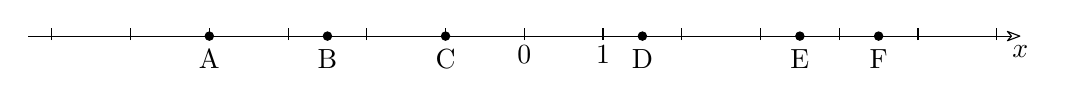
\begin{tikzpicture}[x=10mm, y=10mm, smooth]

%Asse cartesiano con trattini
% (c) 2014 Daniele Zambelli - daniele.zambelli@gmail.com

%%%
% Asse cartesiano con i trattini
%%%%
%Asse cartesiano con trattini
% \usepgflibrary{arrows.meta}

\draw [-{Stealth[length=2mm, open, round]}] (-6.3,0) -- (6.3,0) node [below]  {$x$};
\foreach \xi in {-6, -5, ..., 6}
\draw [-] (\xi, -.05) -- (\xi, .1);
\node [below] at (0, 0) {0};
\node [below] at (1, 0) {1};


\filldraw (-4, 0) circle (1.5pt) node [below, yshift=-.05cm] {A};
\filldraw (-2.5, 0) circle (1.5pt) node [below, yshift=-.05cm] {B};
\filldraw (-1, 0) circle (1.5pt) node [below, yshift=-.05cm] {C};
\filldraw (1.5, 0) circle (1.5pt) node [below, yshift=-.05cm] {D};
\filldraw (3.5, -0) circle (1.5pt) node [below, yshift=-.05cm] {E};
\filldraw (4.5, 0) circle (1.5pt) node [below, yshift=-.05cm] {F};

\end{tikzpicture} \end{center}

  Con riferimento alla figura precedente possiamo dire che:

$x_A=\dots \quad \quad$ $x_B=\dots \quad \quad$ $x_C=\dots \quad \quad$  
$x_D=\dots \quad \quad$ $x_E=\dots \quad \quad$ $x_F=\dots \quad \quad$  
 \end{esempio}
 \begin{esempio}
  \label{ex:D.11}
  Date le coordinate disegna i punti.

  \begin{center} % (c) 2014 Daniele Zambelli - daniele.zambelli@gmail.com

%%%
% Asse cartesiano con i trattini
%%%%
%\usepgflibrary{arrows.meta}
 
\begin{tikzpicture}[x=10mm, y=10mm, smooth]

%Asse cartesiano con trattini
% (c) 2014 Daniele Zambelli - daniele.zambelli@gmail.com

%%%
% Asse cartesiano con i trattini
%%%%
%Asse cartesiano con trattini
% \usepgflibrary{arrows.meta}

\draw [-{Stealth[length=2mm, open, round]}] (-6.3,0) -- (6.3,0) node [below]  {$x$};
\foreach \xi in {-6, -5, ..., 6}
\draw [-] (\xi, -.05) -- (\xi, .1);
\node [below] at (0, 0) {0};
\node [below] at (1, 0) {1};


\end{tikzpicture} \end{center}

  In questo altro asse cartesiano inserisci i seguenti punti:

  $A(7;); \quad B(2;); \quad C(-4;); \quad 
  D(-1;); \quad E(6,5;); \quad F(-5,5;)$.
 \end{esempio}
\end{exrig}

\subsection{Lunghezza di un segmento}

Un primo problema che possiamo affrontare e risolvere avendo un 
riferimento cartesiano è quello di trovare la lunghezza di un segmento
date le coordinate dei suoi estremi. Andiamo per gradi.

\subsubsection*{Primo caso: gli estremi sono entrambi positivi} 

Disegniamo su un asse cartesiano i due punti:~$A(2;)$~e~$B(9;)$.
Il segmento~$AB$ si ottiene togliendo dal segmento~$OB$ il 
segmento~$OA$:~$AB=OB-OA$.

\begin{center} % (c) 2014 Daniele Zambelli - daniele.zambelli@gmail.com

%%%
% Asse cartesiano con alcuni esempi di punti
%%%%
\begin{tikzpicture}[x=5mm, y=5mm, smooth]

% (c) 2014 Daniele Zambelli - daniele.zambelli@gmail.com

%%%
% Asse cartesiano con i trattini
%%%%
%Asse cartesiano con trattini
% \usepgflibrary{arrows.meta}

\draw [-{Stealth[length=2mm, open, round]}] (-12.3, 0) -- (12.3, 0) node [below]  {$x$};
\foreach \xi in {-12, -11, ..., 12}
\draw [-] (\xi, -.05) -- (\xi, .1);
\node [below] at (0, 0) {0};
\node [below] at (1, 0) {1};


% Distanza tra punti entrambi di coordinata positiva
\filldraw (2, 0) circle (1.5pt) node [below, yshift=-.05cm] {A};
\filldraw (9, 0) circle (1.5pt) node [below, yshift=-.05cm] {B};

\end{tikzpicture} \end{center}

Le distanze di~$A$~e~$B$ dall'origine si trovano senza calcoli, sono
proprio le coordinate dei due punti e quindi la distanza di~$A$~da~$B$ si 
ottiene calcolando la differenza delle coordinate di B e di A:

$\overline{AB} = x_B - x_A = 9 - 2 = 7$

Risultato che possiamo verificare facilmente.

\subsubsection*{Secondo caso: gli estremi sono entrambi negativi} 

Consideriamo ora due punti negativi ad esempio:~$A(-8;)$~e~$B(-3;)$. 

\begin{center} % (c) 2014 Daniele Zambelli - daniele.zambelli@gmail.com

%%%
% Asse cartesiano con alcuni esempi di punti
%%%%
\begin{tikzpicture}[x=5mm, y=5mm, smooth]

% (c) 2014 Daniele Zambelli - daniele.zambelli@gmail.com

%%%
% Asse cartesiano con i trattini
%%%%
%Asse cartesiano con trattini
% \usepgflibrary{arrows.meta}

\draw [-{Stealth[length=2mm, open, round]}] (-12.3, 0) -- (12.3, 0) node [below]  {$x$};
\foreach \xi in {-12, -11, ..., 12}
\draw [-] (\xi, -.05) -- (\xi, .1);
\node [below] at (0, 0) {0};
\node [below] at (1, 0) {1};


% Distanza tra punti entrambi di coordinata positiva
\filldraw (-8, 0) circle (1.5pt) node [below, yshift=-.05cm] {A};
\filldraw (-3, 0) circle (1.5pt) node [below, yshift=-.05cm] {B};

\end{tikzpicture} \end{center}

La lunghezza del segmento~AB si ottiene togliendo dalla lunghezza di~AO 
la lunghezza di~BO. La lunghezza di~AO è l'opposto della coordinata di~A 
e la lunghezza di~BO è l'opposto della coordinata di~B, quindi:

$\overline{AB} = (-x_A) - (-x_B) = x_B - x_A = -3 - (-8) = -3 + 8 = 5$

Dopo aver verificato il risultato nel disegno osserviamo che la formula usata 
è identica a quella utilizzata nel caso precedente.

\subsubsection*{Terzo caso: gli estremi sono uno negativo e uno positivo} 

Ora prendiamo un punto negativo e uno positivo:~$A(-5;)$~e~$B(7;)$. 

\begin{center} % (c) 2014 Daniele Zambelli - daniele.zambelli@gmail.com

%%%
% Asse cartesiano con alcuni esempi di punti
%%%%
\begin{tikzpicture}[x=5mm, y=5mm, smooth]

% (c) 2014 Daniele Zambelli - daniele.zambelli@gmail.com

%%%
% Asse cartesiano con i trattini
%%%%
%Asse cartesiano con trattini
% \usepgflibrary{arrows.meta}

\draw [-{Stealth[length=2mm, open, round]}] (-12.3, 0) -- (12.3, 0) node [below]  {$x$};
\foreach \xi in {-12, -11, ..., 12}
\draw [-] (\xi, -.05) -- (\xi, .1);
\node [below] at (0, 0) {0};
\node [below] at (1, 0) {1};


% Distanza tra punti entrambi di coordinata positiva
\filldraw (-5, 0) circle (1.5pt) node [below, yshift=-.05cm] {A};
\filldraw (7, 0) circle (1.5pt) node [below, yshift=-.05cm] {B};

\end{tikzpicture} \end{center}

È chiaro che il segmento~AB si ottiene sommando i due segmenti:~AO~e~OB. 
Ma la lunghezza di~AO è l'opposto della sua coordinata, quindi otteniamo:

$\overline{AB} = -x_A + x_B = x_B - x_A = 7 + 5 = 12$

Anche qui possiamo verificare facilmente il risultato ottenuto.

\subsubsection*{Situazione strana: segmento di lunghezza negativa} 

Abbiamo visto che in tutti questi casi la formula:

$\overline{AB} = x_B - x_A$ funziona quindi non dobbiamo preoccuparci del 
segno delle coordinate per trovare la lunghezza di un segmento facciamo 
sempre la coordinata del secondo punto meno la coordinata del primo.

Ma cosa succede se questa regola la applichiamo al 
segmento:~$A(7;)$~e~$B(2;)$?

\begin{center} % (c) 2014 Daniele Zambelli - daniele.zambelli@gmail.com

%%%
% Asse cartesiano con alcuni esempi di punti
%%%%
\begin{tikzpicture}[x=5mm, y=5mm, smooth]

% (c) 2014 Daniele Zambelli - daniele.zambelli@gmail.com

%%%
% Asse cartesiano con i trattini
%%%%
%Asse cartesiano con trattini
% \usepgflibrary{arrows.meta}

\draw [-{Stealth[length=2mm, open, round]}] (-12.3, 0) -- (12.3, 0) node [below]  {$x$};
\foreach \xi in {-12, -11, ..., 12}
\draw [-] (\xi, -.05) -- (\xi, .1);
\node [below] at (0, 0) {0};
\node [below] at (1, 0) {1};


% Distanza tra punti entrambi di coordinata positiva
\filldraw (7, 0) circle (1.5pt) node [below, yshift=-.05cm] {A};
\filldraw (2, 0) circle (1.5pt) node [below, yshift=-.05cm] {B};

\end{tikzpicture} \end{center}

Applicando la solita regola:
$\overline{AB} = x_B - x_A = 2 - 7 = -5$
otteniamo un numero negativo, strano per una lunghezza! 
I matematici, piuttosto che complicare la formuletta preferiscono dare un 
senso anche alle lunghezze negative parlando di \emph{segmento orientato}.
Un segmento orientato ha lunghezza positiva se il verso del segmento è
uguale al verso del sistema di riferimento, ha lunghezza negativa se
il verso del segmento è opposto a quello del sistema di riferimento.
Qualche volta questo meccanismo può risultare scomodo, in questo caso si 
applica la funzione \emph{valore assoluto} al risultato ottenuto, cioè, se è 
negativo gli si cambia il segno.

\subsection{Punto medio di un segmento}

Un altro problema che possiamo affrontare e risolvere avendo un riferimento 
cartesiano è quello di trovare il punto medio~M date le coordinate degli 
estremi.

Disegniamo su un asse cartesiano i due punti:~$A(3;)$~e~$b(9;)$.

\begin{center} % (c) 2014 Daniele Zambelli - daniele.zambelli@gmail.com

%%%
% Asse cartesiano con alcuni esempi di punti
%%%%
\begin{tikzpicture}[x=5mm, y=5mm, smooth]

% (c) 2014 Daniele Zambelli - daniele.zambelli@gmail.com

%%%
% Asse cartesiano con i trattini
%%%%
%Asse cartesiano con trattini
% \usepgflibrary{arrows.meta}

\draw [-{Stealth[length=2mm, open, round]}] (-12.3, 0) -- (12.3, 0) node [below]  {$x$};
\foreach \xi in {-12, -11, ..., 12}
\draw [-] (\xi, -.05) -- (\xi, .1);
\node [below] at (0, 0) {0};
\node [below] at (1, 0) {1};


% Distanza tra punti entrambi di coordinata positiva
\filldraw (3, 0) circle (1.5pt) node [below, yshift=-.05cm] {A};
\filldraw (9, 0) circle (1.5pt) node [below, yshift=-.05cm] {B};

\end{tikzpicture} \end{center}

Per trovare la coordinata del punto medio dobbiamo sommare alla 
coordinata di~A la lunghezza di metà segmento:

$x_M = x_A + \frac{\overline{AB}}{2}$

Riprendendo la formula precedente:

$x_M = x_A + \frac{x_B - x_A}{2} = \frac{2 x_A + x_B - x_A}{2} = 
\frac{x_A + x_B}{2}$

Detto a parole: \emph{La coordinata del punto medio è uguale alla media delle 
coordinate degli estremi}.

Verifica questa formula con le coppie di punti degli esempi precedenti.

\end{comment}
\section{Piano cartesiano}
\label{sec:04_pianocartesiano}

Abbiamo visto qualche problema sull'asse cartesiano, ma in realtà un solo 
asse non è molto interessante. Se invece prendiamo due assi cartesiani non 
paralleli la situazione diventa più complessa, interessante e divertente.

Due assi non paralleli permettono di realizzare una corrispondenza biunivoca 
tra i punti del piano e le coppie ordinate di numeri: ad ogni punto 
corrisponde una ben precisa coppia di numeri e ad ogni coppia di numeri un 
ben preciso punto. La coppia ordinata di numeri prende il nome di 
\emph{coordinate} del punto.

\begin{inaccessibleblock}[Figura: TODO]
 \begin{figure}[h]
 \centering
 \begin{minipage}[t]{.40\textwidth}
%   \centering% (c) 2014 Daniele Zambelli - daniele.zambelli@gmail.com

%%%
% Asse cartesiano con i trattini
%%%%
%\usepgflibrary{arrows.meta}
 
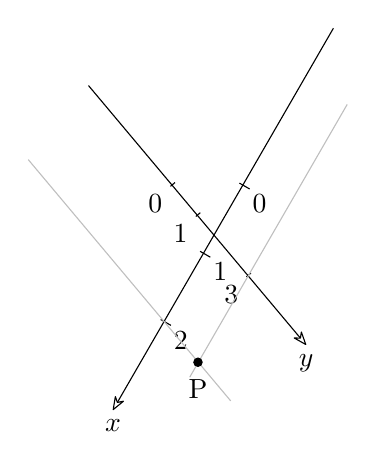
\begin{tikzpicture}[smooth]

%Assi non ortogonali monometrici
\usepgflibrary{arrows.meta}

\begin{scope}[x=10mm, y=10mm, xshift=9mm, rotate=-120]
\draw [-{Stealth[length=2mm, open, round]}] (-2.3, 0) -- (3.3, 0) node [below]  {$x$};
\draw [-] (0, -.05) -- (0, .1) node [below right] at (0, 0) {0};
\draw [-] (1, -.05) -- (1, .1) node [below right] at (1, 0) {1};
\draw [-] (2, -.05) -- (2, .1) node [below right] at (2, 0) {2};
\draw [-] [gray!50, rotate=-20](1.88, -2) -- (1.88, 2);
\end{scope}

\begin{scope}[x=5mm, y=5mm, rotate=-50]
\draw [-{Stealth[length=2mm, open, round]}] (-3.3, 0) -- (5.3, 0) node [below]  {$y$};
\draw [-] (0, -.05) -- (0, .1) node [below left] at (0, 0) {0};
\draw [-] (1, -.05) -- (1, .1) node [below left] at (1, 0) {1};
\draw [-] (3, -.05) -- (3, .1) node [below left] at (3, 0) {3};
\draw [-] [gray!50, rotate=20](2.83, -4) -- (2.83, 4);
\end{scope}

\filldraw (0.33, -2.25) circle (1.5pt) node [below, yshift=-.1cm] {P};

\end{tikzpicture}
  \assistrani
  \caption{Riferimento cartesiano.}\label{fig:assistrani}
 \end{minipage}\hfil
 \begin{minipage}[t]{.50\textwidth}
%   \centering% (c) 2014 Daniele Zambelli - daniele.zambelli@gmail.com

%%%
% Asse cartesiano con i trattini
%%%%
%\usepgflibrary{arrows.meta}
 
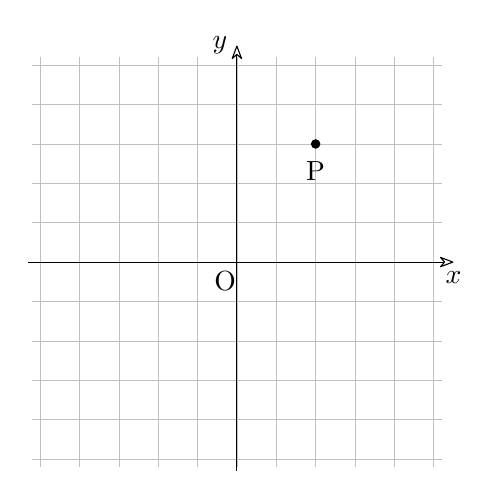
\begin{tikzpicture}[x=5mm, y=5mm, smooth]

%Asse cartesiano con trattini
% (c) 2014 Daniele Zambelli - daniele.zambelli@gmail.com

%%%
% Piano cartesiano: da -5 a +5 scala 0,5
%%%%
% \usepgflibrary{arrows.meta}

% Griglia
\draw[gray!50, very thin, step=1] (-5.2, -5.2) grid (5.2, 5.2);

%Asse x
\draw [-{Stealth[length=2mm, open, round]}] (-5.3,0) -- (5.5,0) node [below]  {$x$};

%Asse y
\draw [-{Stealth[length=2mm, open, round]}] (0, -5.3) -- (0, 5.5) node [left]  {$y$};

\node [below] at (-.3, 0) {O};

\filldraw (2, 3) circle (1.5pt) node [below, yshift=-.1cm] {P};

\end{tikzpicture}
  \assinormali
  \caption{Rif. cart. ortogonale monometrico.}\label{fig:pc}
 \end{minipage}
\end{figure}
\end{inaccessibleblock}

In entrambi questi riferimenti cartesiani al punto~P corrisponde la coppia
di numeri~(2;~3). Pur essendo validi entrambi, per noi sarà molto più comodo 
usare il secondo riferimento cartesiano. Cioè un riferimento in cui gli assi:

\begin{itemize} [noitemsep]
 \item hanno l'origine in comune;
 \item sono perpendicolari;
 \item hanno la stessa unità di misura.
\end{itemize}

Un asse, di solito quello orizzontale, si chiama asse delle \emph{ascisse} 
o asse \emph{x}; l'altro asse di solito quello verticale, si chiama asse 
delle \emph{ordinate} o asse \emph{y}. La prima delle due coordinate
si riferisce alla coordinata dell'asse~$x$, la seconda alla coordinata 
dell'asse~$y$:~$(x;~y)$.

Un riferimento di questo tipo si chiama: 
\emph{Riferimento Cartesiano Ortogonale Monometrico}, (\emph{rcom}). 
E noi d'ora in poi, quando parleremo di piano cartesiano o di riferimento 
cartesiano, ci riferiremo sempre ad un \emph{rcom}.

Riassumendo possiamo dare la seguente definizione:

\begin{definizione}
Si chiama \emph{riferimento cartesiano ortogonale monometrico} 
la coppia di assi cartesiani perpendicolari, con l'origine in comune e 
dotati di uguale unità di misura.
\end{definizione}

Gli assi dividono il piano in quattro zone chiamate quadranti che sono 
numerati come in figura~\ref{fig:quadranti}.

Tutti i punti che appartengono all'asse~$x$ hanno l'ordinata (la~$y$) uguale 
a zero.
Tutti i punti che appartengono all'asse~$y$ hanno l'ascissa (la~$x$) uguale 
a zero.
L'intersezione degli assi, l'origine, ha coordinate~$(0; 0)$

\begin{inaccessibleblock}[Figura: TODO]
 \begin{figure}[h]
 \centering
 \begin{minipage}[t]{.45\textwidth}
%  \centering% (c) 2014 Daniele Zambelli - daniele.zambelli@gmail.com

%%%
% Asse cartesiano con i trattini
%%%%
%\usepgflibrary{arrows.meta}
 
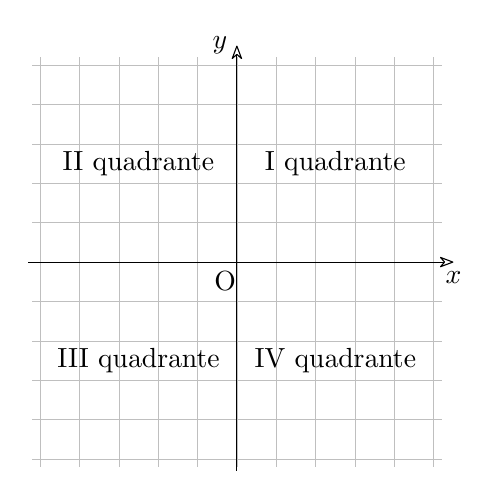
\begin{tikzpicture}[x=5mm, y=5mm, smooth]

%Asse cartesiano con trattini
% (c) 2014 Daniele Zambelli - daniele.zambelli@gmail.com

%%%
% Piano cartesiano: da -5 a +5 scala 0,5
%%%%
% \usepgflibrary{arrows.meta}

% Griglia
\draw[gray!50, very thin, step=1] (-5.2, -5.2) grid (5.2, 5.2);

%Asse x
\draw [-{Stealth[length=2mm, open, round]}] (-5.3,0) -- (5.5,0) node [below]  {$x$};

%Asse y
\draw [-{Stealth[length=2mm, open, round]}] (0, -5.3) -- (0, 5.5) node [left]  {$y$};

\node [below] at (-.3, 0) {O};

\node at (2.5, 2.5) {I quadrante};
\node at (-2.5, 2.5) {II quadrante};
\node at (-2.5, -2.5) {III quadrante};
\node at (2.5, -2.5) {IV quadrante};

\end{tikzpicture}
\pianoconquadranti
 \caption{I quattro quadranti.}\label{fig:quadranti}
 \end{minipage}\hfil
 \begin{minipage}[t]{.45\textwidth}
%  \centering% (c) 2014 Daniele Zambelli - daniele.zambelli@gmail.com

%%%
% Asse cartesiano con i trattini
%%%%
%\usepgflibrary{arrows.meta}
 
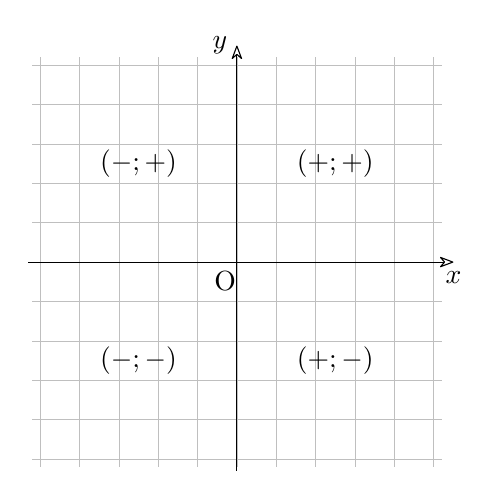
\begin{tikzpicture}[x=5mm, y=5mm, smooth]

%Asse cartesiano con trattini
% (c) 2014 Daniele Zambelli - daniele.zambelli@gmail.com

%%%
% Piano cartesiano: da -5 a +5 scala 0,5
%%%%
% \usepgflibrary{arrows.meta}

% Griglia
\draw[gray!50, very thin, step=1] (-5.2, -5.2) grid (5.2, 5.2);

%Asse x
\draw [-{Stealth[length=2mm, open, round]}] (-5.3,0) -- (5.5,0) node [below]  {$x$};

%Asse y
\draw [-{Stealth[length=2mm, open, round]}] (0, -5.3) -- (0, 5.5) node [left]  {$y$};

\node [below] at (-.3, 0) {O};

\node at (2.5, 2.5) {$(+; +)$};
\node at (-2.5, 2.5) {$(-; +)$};
\node at (-2.5, -2.5) {$(-; -)$};
\node at (2.5, -2.5) {$(+; -)$};

\end{tikzpicture}
\pianoconsegni
 \caption{Collocazione delle coordinate positive e negative.}
 \label{fig:segni}
 \end{minipage}
\end{figure}
\end{inaccessibleblock}

Per rappresentare un punto~$P$ date le sue coordinate~$(x_p; y_p)$ si 
procede nel seguente modo:

\begin{itemize} [noitemsep]
\item determiniamo sull'asse~$x$ il punto~$A$ immagine del numero reale~$x_P~$
\item da~$A$ tracciamo la retta parallela all'asse~$y$
\item determiniamo sull'asse~$y$ il punto~$B$ immagine del numero reale~$y_P~$
\item da~$B$ tracciamo la retta parallela all'asse~$x$.
\end{itemize}

L'intersezione delle parallele tracciate, è il punto~$P$ che ha per coordinate
la coppia ordinata~$(x_P; y_P)$.

Il procedimento inverso permette di passare da un punto del piano alle sue 
coordinate,

\begin{exrig}
\begin{esempio}
 \label{ex:D.12}
  Determiniamo l'immagine delle coppie ordinate~$(2;3)$,~$(-1;4)$,~$(-3;-2)$, 
  e~$(4;-3)$.

  Nella figura~\ref{fig:puntineiquadranti} sono riportati i punti:~$A$ che è 
  l'immagine della coppia~$(2;~3)$, $B$ immagine della coppia~$(-1;~4)$,
  $C$ immagine della coppia~$(3;~-2)$ e $D$ della coppia~$(4;~-3)$.
\end{esempio}

\begin{esempio}
 \label{ex:D.13}
  Determiniamo l'immagine delle seguenti 
  coppie:~$R(0;4)$, $S(0;-2)$, $H(-4;0)$, $K(3;0)$.

  Osserviamo (figura~\ref{fig:puntisugliassi}) che il punto immagine dello zero 
  sull'asse~$x$ coincide con~$O$, quindi la coppia~$(0;~4)$ sarà associata al 
  punto~$R$ dell'asse~$y$ 
  e la coppia~$(0;~-2)$ al punto~$S$ dello stesso asse. 
  Analogamente le coppie~$(-4;~0)$ e~$(3;~0)$ sono associate rispettivamente 
  ai punti~$H$ e~$K$ dell'asse~$x$.
\end{esempio}
 
\begin{inaccessibleblock}[Figura: TODO]
 \begin{figure}[h]
 \centering
 \begin{minipage}[t]{.45\textwidth}
  \centering% (c) 2014 Daniele Zambelli - daniele.zambelli@gmail.com

%%%
% Asse cartesiano con i trattini
%%%%
%\usepgflibrary{arrows.meta}
 
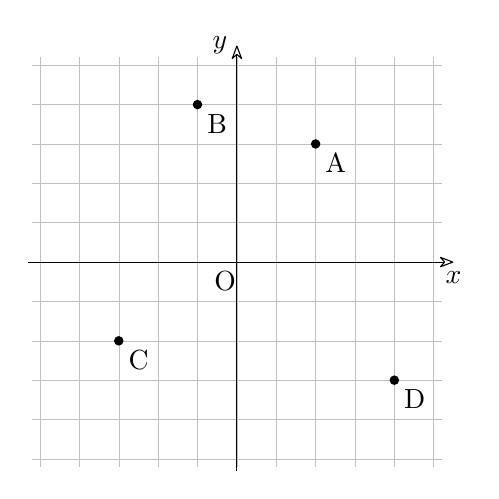
\begin{tikzpicture}[x=5mm, y=5mm, smooth]

%Asse cartesiano con trattini
% (c) 2014 Daniele Zambelli - daniele.zambelli@gmail.com

%%%
% Piano cartesiano: da -5 a +5 scala 0,5
%%%%
% \usepgflibrary{arrows.meta}

% Griglia
\draw[gray!50, very thin, step=1] (-5.2, -5.2) grid (5.2, 5.2);

%Asse x
\draw [-{Stealth[length=2mm, open, round]}] (-5.3,0) -- (5.5,0) node [below]  {$x$};

%Asse y
\draw [-{Stealth[length=2mm, open, round]}] (0, -5.3) -- (0, 5.5) node [left]  {$y$};

\node [below] at (-.3, 0) {O};

\filldraw (2, 3) circle (1.5pt) node [below right] {A};
\filldraw (-1, 4) circle (1.5pt) node [below right] {B};
\filldraw (-3, -2) circle (1.5pt) node [below right] {C};
\filldraw (4, -3) circle (1.5pt) node [below right] {D};

\end{tikzpicture}
  \caption{Punti interni ai quadranti.}\label{fig:puntineiquadranti}
 \end{minipage}\hfil
 \begin{minipage}[t]{.45\textwidth}
  \centering% (c) 2014 Daniele Zambelli - daniele.zambelli@gmail.com

%%%
% Punti appartenenti agli assi
%%%%

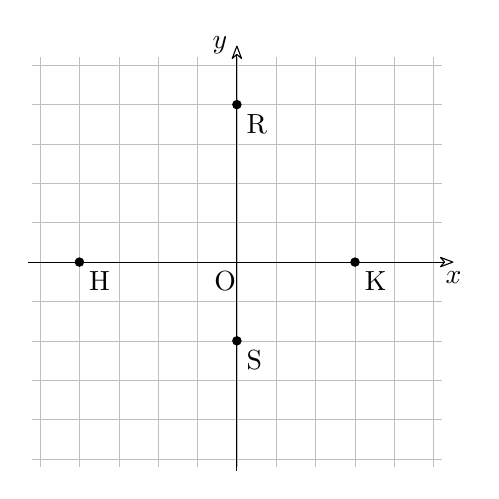
\begin{tikzpicture}[x=5mm, y=5mm, smooth]

% (c) 2014 Daniele Zambelli - daniele.zambelli@gmail.com

%%%
% Piano cartesiano: da -5 a +5 scala 0,5
%%%%
% \usepgflibrary{arrows.meta}

% Griglia
\draw[gray!50, very thin, step=1] (-5.2, -5.2) grid (5.2, 5.2);

%Asse x
\draw [-{Stealth[length=2mm, open, round]}] (-5.3,0) -- (5.5,0) node [below]  {$x$};

%Asse y
\draw [-{Stealth[length=2mm, open, round]}] (0, -5.3) -- (0, 5.5) node [left]  {$y$};

\node [below] at (-.3, 0) {O};


\filldraw (0, 4) circle (1.5pt) node [below right] {R};
\filldraw (0, -2) circle (1.5pt) node [below right] {S};
\filldraw (-4, 0) circle (1.5pt) node [below right] {H};
\filldraw (3, 0) circle (1.5pt) node [below right] {K};

\end{tikzpicture}
  \caption{Punti sugli assi.}\label{fig:puntisugliassi}
 \end{minipage}\hfil
\end{figure}
\end{inaccessibleblock}

\end{exrig}

\section{Problemi nel piano cartesiano}
\label{sec:05_problemipiano}

\subsection{Punto medio di un segmento}

Utilizzando i risultati ottenuti nel caso dei punti posti su un asse 
cartesiano possiamo osservare che anche per quanto riguarda un segmento 
posto nel piano le coordinate del punto medio sono le medie aritmetiche 
delle coordinate degli estremi.

Conoscendo le coordinate degli estremi~$A(x_A; y_A$ e~$B(x_B; y_B)$ 
le coordinate del suo punto medio sono (figura~\ref{fig:puntomedio}):

\begin{inaccessibleblock}[Figura: TODO]
 \begin{figure}[h]
 \centering
 \begin{minipage}[]{.50\textwidth}
  \centering% (c) 2014 Daniele Zambelli - daniele.zambelli@gmail.com

%%%
% Asse cartesiano con i trattini
%%%%
%\usepgflibrary{arrows.meta}
 
\begin{tikzpicture}[x=5mm, y=5mm, smooth]

\clip (-3.5, -1.9) rectangle (10.9, 10.9);

% (c) 2014 Daniele Zambelli - daniele.zambelli@gmail.com

%%%
% Piano cartesiano: da -10 a +10 scala 0,5
%%%%
% \usepgflibrary{arrows.meta}

% Griglia
\draw[gray!50, very thin, step=1] (-10.2, -10.2) grid (10.2, 10.2);

%Asse x
\draw [-{Stealth[length=2mm, open, round]}] (-10.3,0) -- (10.5,0) node [below]  {$x$};

%Asse y
\draw [-{Stealth[length=2mm, open, round]}] (0, -10.3) -- (0, 10.5) node [left]  {$y$};

\node [below] at (-.3, 0) {O};


\coordinate (a) at (2, 3);
\coordinate (b) at (8, 6);
\coordinate (m) at ($ (a)!.5!(b) $);
\draw [-] (a) -- (b);
\filldraw (a) circle (1.5pt) node [below right] {A};
\filldraw (b) circle (1.5pt) node [below right] {B};

\begin{scope}[dotted]
\draw [-] (a) -- (2, 0) node [below] {$x_A$};
\draw [-] (a) -- (0, 3) node [left] {$y_A$};
\draw [-] (b) -- (8, 0) node [below] {$x_B$};
\draw [-] (b) -- (0, 6) node [left] {$y_B$};
\begin{scope}[red]
\filldraw (m) circle (1.5pt) node [below right] {M};
\draw [-] (m) -- (5, 0) node [below] {$\dfrac{x_{A}+x_{B}}{2}$};
\draw [-] (m) -- (0, 4.5) node [left] {$\dfrac{y_{A}+y_{B}}{2}$};
\end{scope}
\end{scope}
\end{tikzpicture}
  \caption{Il punto medio.}\label{fig:puntomedio}
 \end{minipage}
 \begin{minipage}[]{.40\textwidth}
  \[x_{M}=\frac{x_{A}+x_{B}}{2};\, y_{M}=\frac{y_{A}+y_{B}}{2}.\]
  o
  \[M=\left(\dfrac{x_{A}+x_{B}}{2};\, y_{M}=\dfrac{y_{A}+y_{B}}{2} \right).\]
 \end{minipage}
\end{figure}
\end{inaccessibleblock}

\begin{exrig}
 \begin{esempio}
\label{ex:D.18}
  In un piano cartesiano disegna i punti:~$A(-3; -2)$~e~$B(5; 7)$. Trova 
  il punto medio usando il righello disegnalo e assegnagli l'etichetta ``M''.
  Poi calcola le coordinate del punto medio con la formula precedente e 
  controlla che le coordinate ottenute siano proprio quelle del punto trovato 
  precedentemente.
 \end{esempio}

 \begin{esempio}
  In un piano cartesiano disegna i punti:~$A(-9; 8)$~e~$M(-6; 7)$. 
  Usando il righello trova il punto~$B$ in modo che~$M$ sia il punto medio 
  del segmento~$AB$. Applica la formula precedente per verificare la 
  correttezza di quanto trovato.
 \end{esempio}
\end{exrig}

\subsection{Lunghezza di un segmento}

Vogliamo ora determinare la misura~$\overline{AB}$ di un segmento~$AB$, 
date le coordinate degli estremi.

\begin{inaccessibleblock}[Figura: TODO]
 \begin{figure}[h]
 \centering
 \begin{minipage}[t]{.45\textwidth}
  \centering% (c) 2014 Daniele Zambelli - daniele.zambelli@gmail.com

%%%
% Lunghezza di segmenti paralleli agli assi
%%%%

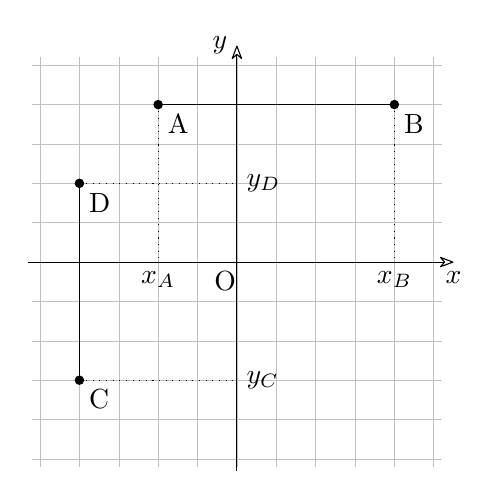
\begin{tikzpicture}[x=5mm, y=5mm, smooth]

% (c) 2014 Daniele Zambelli - daniele.zambelli@gmail.com

%%%
% Piano cartesiano: da -5 a +5 scala 0,5
%%%%
% \usepgflibrary{arrows.meta}

% Griglia
\draw[gray!50, very thin, step=1] (-5.2, -5.2) grid (5.2, 5.2);

%Asse x
\draw [-{Stealth[length=2mm, open, round]}] (-5.3,0) -- (5.5,0) node [below]  {$x$};

%Asse y
\draw [-{Stealth[length=2mm, open, round]}] (0, -5.3) -- (0, 5.5) node [left]  {$y$};

\node [below] at (-.3, 0) {O};


\coordinate (a) at (-2, 4);
\coordinate (b) at (4, 4);
\draw [-] (a) -- (b);
\filldraw (a) circle (1.5pt) node [below right] {A};
\filldraw (b) circle (1.5pt) node [below right] {B};

\begin{scope}[dotted]
\draw [-] (a) -- (-2, 0) node [below] {$x_A$};
\draw [-] (b) -- (4, 0) node [below] {$x_B$};
\end{scope}

\coordinate (c) at (-4, -3);
\coordinate (d) at (-4, 2);
\draw [-] (c) -- (d);
\filldraw (c) circle (1.5pt) node [below right] {C};
\filldraw (d) circle (1.5pt) node [below right] {D};

\begin{scope}[dotted]
\draw [-] (c) -- (0, -3) node [right] {$y_C$};
\draw [-] (d) -- (0, 2) node [right] {$y_D$};
\end{scope}

\end{tikzpicture}
  \caption{Lunghezza segmenti paralleli agli assi.}\label{fig:lungsegpar}
 \end{minipage}\hfil
 \begin{minipage}[t]{.45\textwidth}
  \centering% (c) 2014 Daniele Zambelli - daniele.zambelli@gmail.com

%%%
% Lunghezza di un segmento
%%%%

\begin{tikzpicture}[x=5mm, y=5mm, smooth]

% (c) 2014 Daniele Zambelli - daniele.zambelli@gmail.com

%%%
% Piano cartesiano: da -5 a +5 scala 0,5
%%%%
% \usepgflibrary{arrows.meta}

% Griglia
\draw[gray!50, very thin, step=1] (-5.2, -5.2) grid (5.2, 5.2);

%Asse x
\draw [-{Stealth[length=2mm, open, round]}] (-5.3,0) -- (5.5,0) node [below]  {$x$};

%Asse y
\draw [-{Stealth[length=2mm, open, round]}] (0, -5.3) -- (0, 5.5) node [left]  {$y$};

\node [below] at (-.3, 0) {O};


\coordinate (e) at (-3, -1);
\coordinate (f) at (2, 4);
\coordinate (g) at (2, -1);
\draw [-] (e) -- (f);
\filldraw (e) circle (1.5pt) node [below right] {E};
\filldraw (f) circle (1.5pt) node [below right] {F};
\filldraw (g) circle (1.5pt) node [below right] {G};

\begin{scope}[dotted]
\draw [-] (e) -- (g) node [below, xshift=1mm] at ($(e)!.5!(g)$) {$x_F - x_E$};
\draw [-] (f) -- (g) node [below, xshift=8mm] at ($(f)!.5!(g)$) {$y_F - y_E$};
\end{scope}

\end{tikzpicture}
  \caption{Lunghezza di un segmento.}\label{fig:lungseg}
 \end{minipage}\hfil
\end{figure}
\end{inaccessibleblock}

Possiamo distinguere due casi:

\subsection*{Primo caso: segmenti paralleli agli assi} i due punti hanno la 
stessa ascissa o la stessa ordinata (figura~\ref{fig:lungsegpar}). 
È facile osservare in questo caso che il problema si riduce a quello analogo
risolto per segmenti su un asse cartesiano. Se i due punti hanno la stessa 
ordinata, la stessa~$y$:

$\overline{AB} = x_B - x_A$.

Se hanno la stessa ascissa, la stessa~$x$:

$\overline{CD} = y_D - y_C$.

\subsection*{Secondo caso: segmento qualunque} è questo il caso generale, 
il segmento ha una 
direzione diversa da quella degli assi coordinati (figura~\ref{fig:lungseg}).

\emph{Dati}:~$E(x_E; y_E)$, $F(x_F;y_F)$.

\emph{Obiettivo}:~$\overline{EF}$.

\emph{Procedura risolutiva}: tracciando da~$E$ la parallela all'asse~$x$ 
e da~$F$ la parallela all'asse~$y$ si determina il vertice~$G$ del triangolo 
rettangolo~$EGF$ di cui~$EF$ è l'ipotenusa.
Per il teorema di Pitagora si 
ottiene:~$\overline{EF}=\sqrt{\overline{EG}^2 + \overline{GF}^2}=
\sqrt{\left(x_E-x_G \right)^2+\left(y_G-y_F \right)^2}$. %----figura18

Poiché $x_{G}=x_{F}$ e~$y_{G}=y_{E}$ sostituendo si ha:
$\overline{AB}=\sqrt{\left(x_{E}-x_{F}\right)^{2}+\left(y_{E}-y_{F}\right)^{2}}$.

In conclusione, la \emph{misura del segmento} $AB$, \emph{note le coordinate} 
dei suoi estremi è:

\[\overline{EF}=\sqrt{\left(x_{E}-x_{F}\right)^{2}+\left(y_{E}-y_{F}\right)^{2}}.\]


\subsection{Area sottesa a un segmento}

Dati gli estremi di un segmento trovare la superficie compresa tra il 
segmento e l'asse~$x$. Partiamo da una situazione particolare:
i punti~$A$~e~$B$ non appartengono all'asse~$x$ e il segmento~$AB$ non 
è parallelo all'asse~$x$.

\begin{center} % (c) 2014 Daniele Zambelli - daniele.zambelli@gmail.com

%%%
% Area sottesa a un segmento
%%%%
 
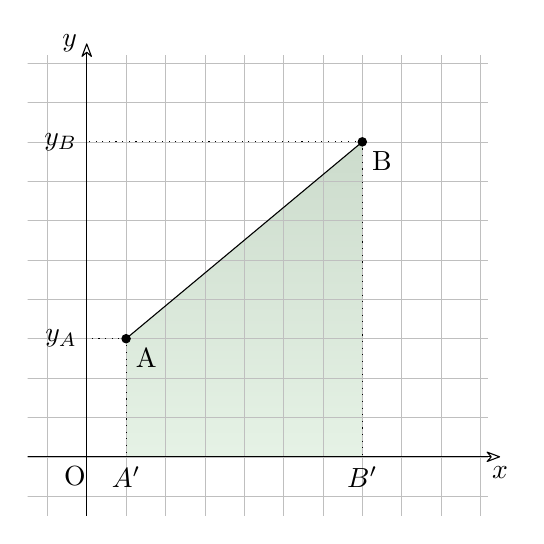
\begin{tikzpicture}[x=5mm, y=5mm, smooth]

\clip (-1.5, -1.5) rectangle (10.9, 10.9);

\coordinate (a) at (1, 3);
\coordinate (xa) at (1, 0);
\coordinate (ya) at (0, 3);
\coordinate (b) at (7, 8);
\coordinate (xb) at (7, 0);
\coordinate (yb) at (0, 8);

\fill [top color=green!30!black!20,bottom color=green!50!black!10] 
 (a) -- (b) -- (xb) -- (xa) -- cycle;

% (c) 2014 Daniele Zambelli - daniele.zambelli@gmail.com

%%%
% Piano cartesiano: da -10 a +10 scala 0,5
%%%%
% \usepgflibrary{arrows.meta}

% Griglia
\draw[gray!50, very thin, step=1] (-10.2, -10.2) grid (10.2, 10.2);

%Asse x
\draw [-{Stealth[length=2mm, open, round]}] (-10.3,0) -- (10.5,0) node [below]  {$x$};

%Asse y
\draw [-{Stealth[length=2mm, open, round]}] (0, -10.3) -- (0, 10.5) node [left]  {$y$};

\node [below] at (-.3, 0) {O};


\draw [-] (a) -- (b);
\filldraw (a) circle (1.5pt) node [below right] {A};
\filldraw (b) circle (1.5pt) node [below right] {B};

\begin{scope}[dotted]
\draw [-] (a) -- (xa) node [below] {$A'$};
\draw [-] (a) -- (ya) node [left] {$y_A$};
\draw [-] (b) -- (xb) node [below] {$B'$};
\draw [-] (b) -- (yb) node [left] {$y_B$};
\end{scope}

\end{tikzpicture} \end{center}

Che forma ha l'area sottesa a questo segmento? È un quadrilatero, ha solo due 
lati paralleli ha due angoli retti... questa è la descrizione di un trapezio!
Forse non hai mai disegnato un trapezio messo in questo modo. Puoi verificare 
facilmente che è un trapezio, ti basta ruotare il quaderno do 90°. 
L'area del trapezio è uguale alla somma delle basi per l'altezza diviso due:

\[Area_{trapezio}= \frac{(B+b)h}{2}\]

Ma quali sono le basi e quale è l'altezza? Nel trapezio le basi sono i due 
lati paralleli e l'altezza è la distanza tra i due lati paralleli.
Uno dei lati paralleli è~$AA'$ cioè l'ordinata di~$A$ (la~$y_A$) 
e l'altro è~$BB'$ cioè l'ordinata di~$B$ (la~$y_B$).
L'altezza del trapezio è la lunghezza del segmento~$A'B'$ 
cioè~$x_B - x_A$.

Mettendo assieme tutti gli ingredienti otteniamo che l'area sottesa al 
segmento~$AB$ è:

\[\mathcal{A}_{AB} = \frac{(y_B + y_A) (x_B - x_A)}{2}\]

E se il segmento è messo in un altro modo?
Anche limitandoci al primo quadrante possiamo osservare che ci sono svariati casi:

\begin{center} % (c) 2014 Daniele Zambelli - daniele.zambelli@gmail.com

%%%
% Aree sottese a diversi segmenti
%%%%
%\usepgflibrary{arrows.meta}
 
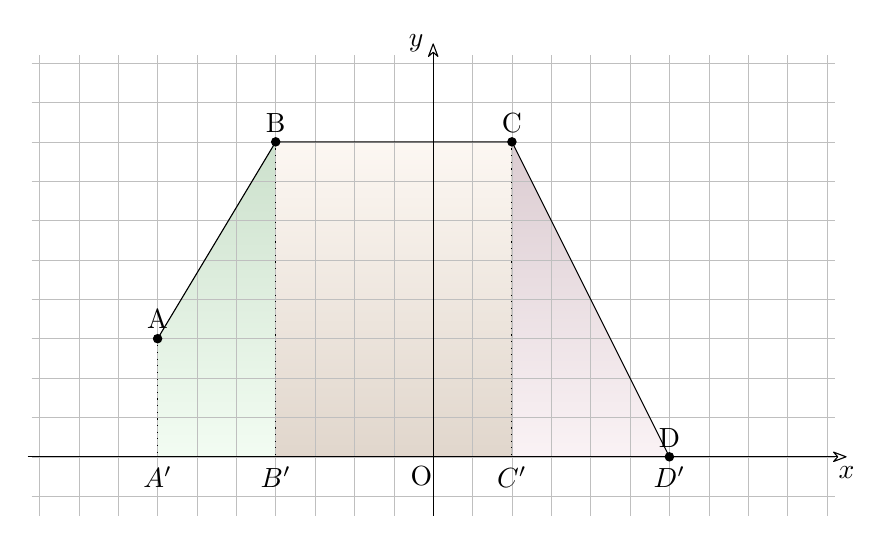
\begin{tikzpicture}[x=5mm, y=5mm, smooth]

\clip (-10.3, -1.5) rectangle (10.9, 10.9);

\coordinate (a) at (-7, 3);
\coordinate (xa) at (-7, 0);
\coordinate (b) at (-4, 8);
\coordinate (xb) at (-4, 0);
\coordinate (c) at (2, 8);
\coordinate (xc) at (2, 0);
\coordinate (d) at (6, 0);
\coordinate (xd) at (6, 0);

\fill [top color=green!40!black!20,bottom color=green!80!black!05] 
 (a) -- (b) -- (xb) -- (xa) -- cycle;
\fill [top color=orange!80!black!05,bottom color=orange!40!black!20] 
 (b) -- (c) -- (xc) -- (xb) -- cycle;
\fill [top color=purple!40!black!20,bottom color=purple!80!black!05] 
 (c) -- (d) -- (xd) -- (xc) -- cycle;

% (c) 2014 Daniele Zambelli - daniele.zambelli@gmail.com

%%%
% Piano cartesiano: da -10 a +10 scala 0,5
%%%%
% \usepgflibrary{arrows.meta}

% Griglia
\draw[gray!50, very thin, step=1] (-10.2, -10.2) grid (10.2, 10.2);

%Asse x
\draw [-{Stealth[length=2mm, open, round]}] (-10.3,0) -- (10.5,0) node [below]  {$x$};

%Asse y
\draw [-{Stealth[length=2mm, open, round]}] (0, -10.3) -- (0, 10.5) node [left]  {$y$};

\node [below] at (-.3, 0) {O};


\draw [-] (a) -- (b) --(c) --(d);
\filldraw (a) circle (1.5pt) node [above] {A};
\filldraw (b) circle (1.5pt) node [above] {B};
\filldraw (c) circle (1.5pt) node [above] {C};
\filldraw (d) circle (1.5pt) node [above] {D};

\begin{scope}[dotted]
\draw [-] (a) -- (xa) node [below] {$A'$};
\draw [-] (b) -- (xb) node [below] {$B'$};
\draw [-] (c) -- (xc) node [below] {$C'$};
\draw [-] (d) -- (xd) node [below] {$D'$};
\end{scope}

\end{tikzpicture} \end{center}

L'area sottesa al segmento~$AB$ è un trapezio rettangolo, 
l'area sottesa al segmento~$CD$ è un rettangolo, 
l'area sottesa al segmento~$EF$ è un triangolo rettangolo.

Nel paragrafo precedente abbiamo risolto il primo caso, quello del trapezio,
dovremo ripetere tutti quei ragionamenti anche per gli altri due? No! 
I matematici, che sono un po strani, ritengono che:

\begin{itemize} [noitemsep]
 \item 
  un triangolo rettangolo
  non sia altro che un trapezio rettangolo con una base lunga zero;
 \item 
  un rettangolo
  non sia altro che un trapezio rettangolo con le basi uguali.
\end{itemize}

A questo punto non dobbiamo preoccuparci di casi diversi, la formula trovata 
per il trapezio rettangolo risolverà anche gli altri casi

\begin{exrig}
 \begin{esempio}
\label{ex:D.18}
  Dopo aver trovato le coordinate dei punti della figura precedente calcola
  le aree sottese ai tre segmenti sia usando le formule della geometria
  sia usando la formula dell'area sottesa e confronta i risultati.
 \end{esempio}

 \begin{esempio}
  In un piano cartesiano disegna i punti:~$A(3; -2)$~e~$B(8; -6)$. 
  Calcola l'area sottesa a questo segmento sia usando la formula 
  dell'area del trapezio sia usando la formula dell'area sottesa...
  Cosa puoi osservare?
 \end{esempio}
\end{exrig}

Anche per le aree sottese abbiamo una situazione strana: in certi casi 
l'area di una figura risulta negativa. Questo fatto può essere irritante, 
ma in certi casi risulterà comodo.

Ci sono certi segmenti che formano con l'asse~$x$ una figura con una 
superficie diversa da zero ma che hanno area sottesa uguale a zero.
Quando avviene questo?

\subsection{Area di un triangolo}

Date le coordinate dei vertici di un triangolo trova l'area della sua 
superficie.

\begin{inaccessibleblock}[Figura: TODO]
 \begin{figure}[h]
 \centering
 \begin{minipage}[t]{.45\textwidth}
  \centering% (c) 2014 Daniele Zambelli - daniele.zambelli@gmail.com

%%%
% Aree di un triangolo con la formula di Erone
%%%%
 
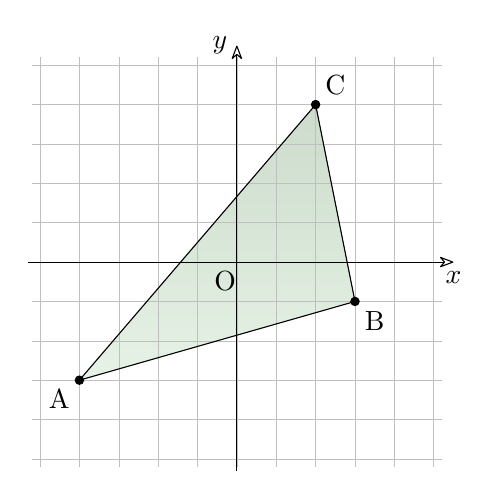
\begin{tikzpicture}[x=5mm, y=5mm, smooth]

%\clip (-10.3, -1.5) rectangle (10.9, 10.9);

\coordinate (a) at (-4, -3);
\coordinate (b) at (3, -1);
\coordinate (c) at (2, 4);

\fill [top color=green!30!black!20,bottom color=green!50!black!10] 
 (a) -- (b) -- (c) -- cycle;

% (c) 2014 Daniele Zambelli - daniele.zambelli@gmail.com

%%%
% Piano cartesiano: da -5 a +5 scala 0,5
%%%%
% \usepgflibrary{arrows.meta}

% Griglia
\draw[gray!50, very thin, step=1] (-5.2, -5.2) grid (5.2, 5.2);

%Asse x
\draw [-{Stealth[length=2mm, open, round]}] (-5.3,0) -- (5.5,0) node [below]  {$x$};

%Asse y
\draw [-{Stealth[length=2mm, open, round]}] (0, -5.3) -- (0, 5.5) node [left]  {$y$};

\node [below] at (-.3, 0) {O};


\draw [-] (a) -- (b) --(c) -- cycle;
\filldraw (a) circle (1.5pt) node [below left] {A};
\filldraw (b) circle (1.5pt) node [below right] {B};
\filldraw (c) circle (1.5pt) node [above right] {C};

\end{tikzpicture}
  \caption{Area con la formula di Erone.}\label{fig:triangoloerone}
 \end{minipage}\hfil
 \begin{minipage}[t]{.45\textwidth}
  \centering% (c) 2014 Daniele Zambelli - daniele.zambelli@gmail.com

%%%
% Aree di un triangolo ottenuta come differenza di aree
%%%%
 
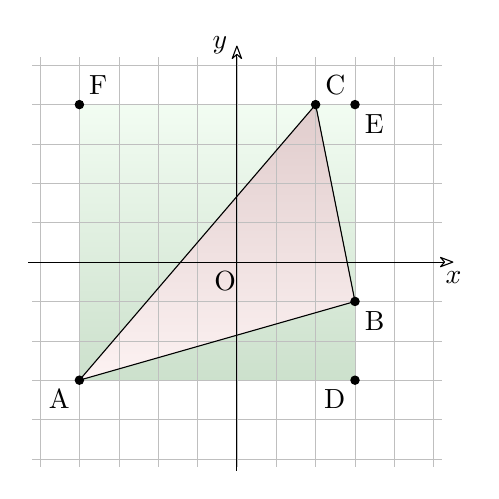
\begin{tikzpicture}[x=5mm, y=5mm, smooth]

\coordinate (a) at (-4, -3);
\coordinate (b) at (3, -1);
\coordinate (c) at (2, 4);
\coordinate (d) at (3, -3);
\coordinate (e) at (3, 4);
\coordinate (f) at (-4, 4);

\fill [top color=green!80!black!05,bottom color=green!40!black!20] 
 (a) -- (d) -- (e) -- (f) -- cycle;

\fill [top color=red!40!black!20,bottom color=red!80!black!05] 
 (a) -- (b) -- (c) -- cycle;

% (c) 2014 Daniele Zambelli - daniele.zambelli@gmail.com

%%%
% Piano cartesiano: da -5 a +5 scala 0,5
%%%%
% \usepgflibrary{arrows.meta}

% Griglia
\draw[gray!50, very thin, step=1] (-5.2, -5.2) grid (5.2, 5.2);

%Asse x
\draw [-{Stealth[length=2mm, open, round]}] (-5.3,0) -- (5.5,0) node [below]  {$x$};

%Asse y
\draw [-{Stealth[length=2mm, open, round]}] (0, -5.3) -- (0, 5.5) node [left]  {$y$};

\node [below] at (-.3, 0) {O};


\draw [-] (a) -- (b) --(c) -- cycle;
\filldraw (a) circle (1.5pt) node [below left] {A};
\filldraw (b) circle (1.5pt) node [below right] {B};
\filldraw (c) circle (1.5pt) node [above right] {C};
\filldraw (d) circle (1.5pt) node [below left] {D};
\filldraw (e) circle (1.5pt) node [below right] {E};
\filldraw (f) circle (1.5pt) node [above right] {F};

\end{tikzpicture}
  \caption{Area come differenza di superfici.}\label{fig:triangolodifferenza}
 \end{minipage}\hfil
\end{figure}
\end{inaccessibleblock}

\subsection*{Formula di Erone}
Se conosciamo le coordinate dei tre vertici possiamo trovare le lunghezze dei 
tre lati e conoscendo le lunghezze dei lati di un triangolo possiamo trovare
la sua area utilizzando la formula di Erone. Chiamando:~$a$,~$b$~e~$c$ i tre 
lati e~$p$ il semiperimetro:

\[\mathcal{A}_{triangolo} = \sqrt{p(p-a)(p-b)(p-c)}\]

Ma spesso le lunghezze dei lati sono numeri approssimati e quindi la formula
di Erone, già complicata di suo, risulta piuttosto scomoda.

\subsection*{Differenza di superfici}
Un altro metodo consiste nell'iscrivere il triangolo in un rettangolo, 
trovare l'area del rettangolo e sottrarre da questa le aree dei tre triangoli 
complementari.

\[\mathcal{A}_{triangolo} = \mathcal{A}_{rettangolo}-\mathcal{A}_{tri1}
                                                    -\mathcal{A}_{tri2}
                                                    -\mathcal{A}_{tri3}\]

\subsection*{Casi particolari}

\begin{inaccessibleblock}[Figura: TODO]
 \begin{figure}[h]
 \centering
 \begin{minipage}[t]{.45\textwidth}
  \centering% (c) 2014 Daniele Zambelli - daniele.zambelli@gmail.com

%%%
% Aree di un triangolo con la formula di Erone
%%%%
 
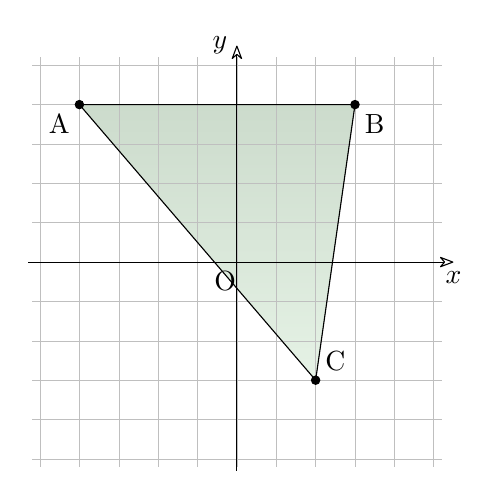
\begin{tikzpicture}[x=5mm, y=5mm, smooth]

%\clip (-10.3, -1.5) rectangle (10.9, 10.9);

\coordinate (a) at (-4, 4);
\coordinate (b) at (3, 4);
\coordinate (c) at (2, -3);

\fill [top color=green!30!black!20,bottom color=green!50!black!10] 
 (a) -- (b) -- (c) -- cycle;

% (c) 2014 Daniele Zambelli - daniele.zambelli@gmail.com

%%%
% Piano cartesiano: da -5 a +5 scala 0,5
%%%%
% \usepgflibrary{arrows.meta}

% Griglia
\draw[gray!50, very thin, step=1] (-5.2, -5.2) grid (5.2, 5.2);

%Asse x
\draw [-{Stealth[length=2mm, open, round]}] (-5.3,0) -- (5.5,0) node [below]  {$x$};

%Asse y
\draw [-{Stealth[length=2mm, open, round]}] (0, -5.3) -- (0, 5.5) node [left]  {$y$};

\node [below] at (-.3, 0) {O};


\draw [-] (a) -- (b) --(c) -- cycle;
\filldraw (a) circle (1.5pt) node [below left] {A};
\filldraw (b) circle (1.5pt) node [below right] {B};
\filldraw (c) circle (1.5pt) node [above right] {C};

\end{tikzpicture}
  \caption{Area con la formula di Erone.}\label{fig:triangoloparallelox}
 \end{minipage}\hfil
 \begin{minipage}[t]{.45\textwidth}
  \centering% (c) 2014 Daniele Zambelli - daniele.zambelli@gmail.com

%%%
% Aree di un triangolo con la formula di Erone
%%%%
 
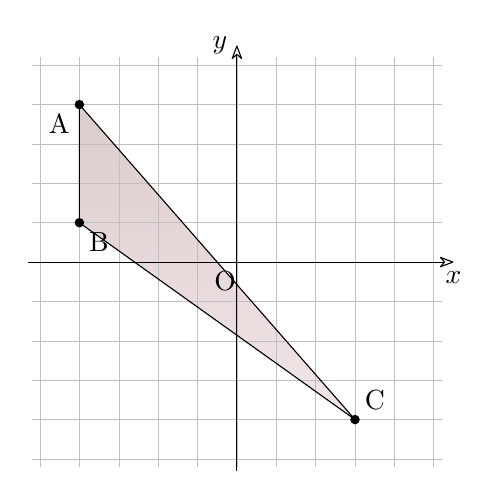
\begin{tikzpicture}[x=5mm, y=5mm, smooth]

%\clip (-10.3, -1.5) rectangle (10.9, 10.9);

\coordinate (a) at (-4, 4);
\coordinate (b) at (-4, 1);
\coordinate (c) at (3, -4);

\fill [top color=red!30!black!20,bottom color=red!50!black!10] 
 (a) -- (b) -- (c) -- cycle;

% (c) 2014 Daniele Zambelli - daniele.zambelli@gmail.com

%%%
% Piano cartesiano: da -5 a +5 scala 0,5
%%%%
% \usepgflibrary{arrows.meta}

% Griglia
\draw[gray!50, very thin, step=1] (-5.2, -5.2) grid (5.2, 5.2);

%Asse x
\draw [-{Stealth[length=2mm, open, round]}] (-5.3,0) -- (5.5,0) node [below]  {$x$};

%Asse y
\draw [-{Stealth[length=2mm, open, round]}] (0, -5.3) -- (0, 5.5) node [left]  {$y$};

\node [below] at (-.3, 0) {O};


\draw [-] (a) -- (b) --(c) -- cycle;
\filldraw (a) circle (1.5pt) node [below left] {A};
\filldraw (b) circle (1.5pt) node [below right] {B};
\filldraw (c) circle (1.5pt) node [above right] {C};

\end{tikzpicture}
  \caption{Area come differenza di superfici.}\label{fig:triangoloparalleloy}
 \end{minipage}\hfil
\end{figure}
\end{inaccessibleblock}

Se il triangolo ha un lato parallelo ad uno degli assi allora è facile 
calcolare l'altezza rispetto a questo lato e quindi si può usare la 
solita formula:

\[\mathcal{A}_{triangolo} = \frac{b \cdot h}{2}\]

\begin{exrig}
 Dopo aver trovato le coordinate dei vertici delle figure precedenti:

 \begin{esempio}
 \label{ex:D.18}
  Con riferimento alla figura~\ref{fig:triangoloerone} calcola 
  la lunghezza dei lati e l'area del triangolo con la formula di Erone.
 \end{esempio}

 \begin{esempio}
  Con riferimento alla figura~\ref{fig:triangolodifferenza} calcola 
  l'area del triangolo come differenza di aree.
  Confronta poi il risultato con quello ottenuto nel calcolo precedente.
 \end{esempio}

 \begin{esempio}
  Con riferimento alla figura~\ref{fig:triangoloparallelox} calcola 
  l'area del triangolo in due modi diversi e confronta i risultati.
 \end{esempio}

 \begin{esempio}
  Con riferimento alla figura~\ref{fig:triangoloparalleloy} calcola 
  l'area del triangolo in due modi diversi e confronta i risultati.
 \end{esempio}
\end{exrig}

% \newpage
% \input{./02_01_pianocartesiano_ese}
% \cleardoublepage
